
%!TEX root = ../article.tex

% Relatedwork
\section{Related Work}
\label{related work}


\subsection{Failue detection technology in distributed system}
Paul Stelling et al.\cite{zou2014improving} proposed a fault detection service which use techniques based on unreliable fault detectors to detect and report component failure for high-performance distributed computing systems,while allowing the user to trade off timeliness of reporting against false postive.
Marin BERTIER et al.\cite{bertier2003performance}  present a failure detector implementation, in which a variant of the heartbeat failure detector, is both adaptable and designed for scalability.
Naohiro Hayashibara et al.\cite{hayashibara2002failure} identified problems for designing and implementing a scalable and generic failure detector service in a Grid system.in their paper, they describe some of the proposed protocols for failure detection and discuss their effectiveness and how they address the identified problems
Chinghway Lim et al.\cite{lim2008log} showed a approach which is to transform the chaotic log files into a standard form for visualization,Together with user feedback and simple analysis tools, visualization allowed expert knowledge to be efficiently applied to anomaly prediction, detection and
categorization.the analysis techniques in his paper led to the detection and categorization of several failure types and in some cases
predicted trends which lead towards failures.
Weiwei Shi et al.\cite{shi2016integrated} propose an improved data preprocessing framework DPF on Apache Spark for missing data prediction and fault type diagnose incorporating optimized LinR,data fusion and data cleansing to improve the quality of raw data generated by State Grid of China.
Kenji Yamanishi et al.\cite{yamanishi2005dynamic} used Syslog monitoring technologies to address a wide range of important issues including network failure symptom detection and event correlation discovery,in their paper,a new methodology of dynamic syslog mining was proposed in order to detect failure symptoms with higher confidence and to discover sequential alarm patterns among computer devices
\subsection{Fault Diagnosis related research on cloud platform}
Jia Tong et al.\cite{tong2016approach} present an approach to pinpoint bug-induced failue in logs for open cloud platforms,two algorithms called MPIN and SPIN are used in the paper to generate a predictive model based on log vectors.
Jianwen WEI et al.\cite{wei2011analysis} proposed a scalable platform for network log analysis, which targets for fast aggregation and agile query
[Cloud and Virtualization Based Log Management Service]
Sai Rakesh Ghanta et al.\cite{ghanta2017cloud} presented a solution that integrates some of the newest and popular open-source technologies, to tackle the problems that many enterprises are facing in log management
Saibharath S et al.\cite{saibharath2014design} developed a forensic framework to do cloud forensics in OpenStack for infrastructure
as a service model using the existing forensic tools
\subsection{Log mining for cloud platform}
Meera G et al.\cite{meera2016event} discusses event correlation techniques to group events logged by OpenStack tenants of interest,which ensures that the investigator views only information relevant to the tenant under suspicion
Pooya Musavi et al.\cite{Musavi2016Reliabiligy} conducted an empirical study to investigate the API failures in a cloud environment by mining bugs of 25 modules within the 5 most important OpenStack APIs.Decision Trees to build their models, but other techniques such as Support Vector Machines (SVM) and Logistics Regression should be studied and compared.
Extracting fault features with the error logs of fault injection tests has been widely studied in the area of large scale distributed systems for decades
Xiang Rao et al.\cite{rao2011identifying} present a similarity-based error log filtering method SBF to filter out noisy error logs and  increase the precision and the recall rate of fault feature extraction.
Deqing Zou et al.\cite{zou2014improving} presents a UiLog system for fault analysis and diagnosis,which collect the system log information of each component and track logs for statistics,and they proposed a Fault Keyword matrix analysis technology to classify log into different catalogues according to different fault types.
Byung Chul Tak et al.\cite{tak2016logan} presented a log analysis tool LOGAN for problem diagnosis in cloud platform,they design and develop some log correlation techniques, log comparison using templates and intuitive visualization modules.
Xiwei Xu et al.\cite{xu2014pod} we propose Process Oriented Dependability (POD)-Diagnosis, an approach that explicitly models these sporadic operations as processes. 
\subsection{ELK Stack}
ELK (Elastic Search,LogStash,Kibana) could be used as a log management system which is very convenient for user to interpret and insight the result. FigX shows the overview framework of ELK. 
Elasticsearch is a real-time distributed search and analytics engine. It allows you to explore your data at a speed and at a scale never before possible. It is used for full-text search, structured search, analytics\cite{ELKIntro2017}. Logstash is the central dataflow engine in the Elastic Stack for gathering, enriching, and unifying all of your data regardless of format or schema\cite{ELKIntro2017}.Kibana is a window into the Elastic Stack. It enables visual exploration and real-time analysis of your data in Elasticsearch\cite{ELKIntro2017}.
\begin{figure}[!h]
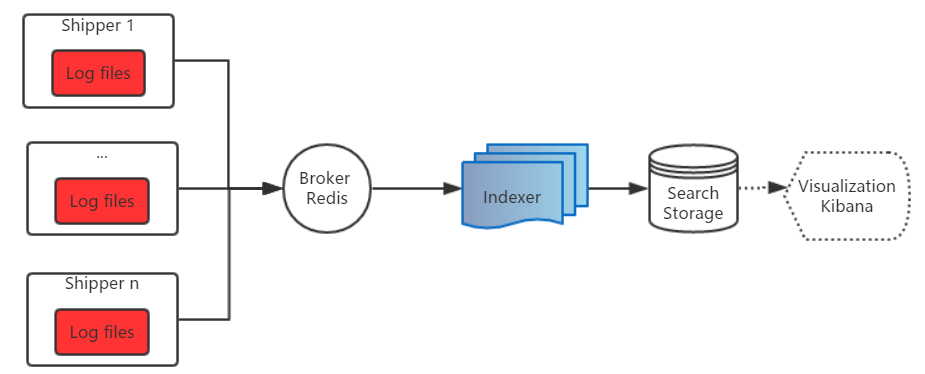
\includegraphics[scale=0.5]{./figures/Fig2.png} 
\caption{Overview of ELK Stack}
\end{figure}

